% ------------------------------------------------------------------------------
% Risk Modeller's Toolkit (RMTK) User Guide
%
% Authors:
% 	V. Silva, C. Casotto, A. Rao, M. Villar, H. Crowley	- GEM Model Facility, Pavia, Italy
%   D. Vamvatsikos
%
%
% License:
% Document distributed under the CC BY-NC-SA 4.0 License
% Creative Commons Attribution-NonCommercial-ShareAlike 4.0 International
% http://creativecommons.org/licenses/by-nc-sa/4.0/
%
% Copyright:
% © GEM Foundation, Pavia, Italy. July 2015.
% ------------------------------------------------------------------------------

%-------------------------------------------------------------------------------
%  PACKAGES AND OTHER DOCUMENT CONFIGURATIONS
%-------------------------------------------------------------------------------

\documentclass[11pt,fleqn]{book} % ------------------ Left-justified equations -
%%%%%%%%%%%%%%%%%%%%%%%%%%%%%%%%%%%%%%%%%
% The Legrand Orange Book
% LaTeX Template
% Version 1.4 (12/4/14)
%
% This template has been downloaded from:
% http://www.LaTeXTemplates.com
%
% Original author:
% Mathias Legrand (legrand.mathias@gmail.com)
%
% License:
% CC BY-NC-SA 3.0 (http://creativecommons.org/licenses/by-nc-sa/3.0/)
%
% Compiling this template:
% This template uses biber for its bibliography and makeindex for its index.
% When you first open the template, compile it from the command line with the 
% commands below to make sure your LaTeX distribution is configured correctly:
%
% 1) pdflatex oq-manual
% 2) makeindex oq-manual.idx -s StyleInd.ist
% 3) biber oq-manual
% 4  makeglossaries oq-manual
% 4) pdflatex oq-manual x 2
%
% After this, when you wish to update the bibliography/index use the appropriate
% command above and make sure to compile with pdflatex several times 
% afterwards to propagate your changes to the document.
%
% This template also uses a number of packages which may need to be
% updated to the newest versions for the template to compile. It is strongly
% recommended you update your LaTeX distribution if you have any
% compilation errors.
%
% Important note:
% Chapter heading images should have a 2:1 width:height ratio,
% e.g. 920px width and 460px height.
%
%%%%%%%%%%%%%%%%%%%%%%%%%%%%%%%%%%%%%%%%%
\usepackage[top=3cm,bottom=3cm,left=3.2cm,right=3.2cm,headsep=10pt,a4paper]{geometry} % Page margins

\usepackage{xcolor} % Required for specifying colors by name
\definecolor{ocre}{RGB}{243,102,25} % Define the orange color used for highlighting throughout the book

% Font Settings
\usepackage{avant} % Use the Avantgarde font for headings
%\usepackage{times} % Use the Times font for headings
\usepackage{mathptmx} % Use the Adobe Times Roman as the default text font together with math symbols from the Sym­bol, Chancery and Com­puter Modern fonts

\usepackage{microtype} % Slightly tweak font spacing for aesthetics
\usepackage[utf8]{inputenc} % Required for including letters with accents
\usepackage[T1]{fontenc} % Use 8-bit encoding that has 256 glyphs

% Bibliography
\usepackage{csquotes}
\usepackage[style=alphabetic,
            sorting=nyt,
            sortcites=true,
            natbib=true,
            style=authoryear,
            maxcitenames=2,
            maxbibnames=100,
            autopunct=true,
            babel=hyphen,
            hyperref=true,
            doi=true,
            abbreviate=false,
            backref=true,
            backend=bibtex,
	    	uniquename=false,
	    	uniquelist=false]{biblatex}
\addbibresource{./bibliography/hazard.bib} % BibTeX bibliography file
\addbibresource{./bibliography/risk.bib} % BibTeX bibliography file
\defbibheading{bibempty}{}

% Figure caption settings
\usepackage[textfont=it,margin=10pt,font=small,labelfont=bf,labelsep=endash]{caption}
\usepackage{subcaption}
\usepackage{rotating}

% Table - colors from
\usepackage{verbatim}
\usepackage{fancyvrb}
\usepackage{color, colortbl}
\definecolor{darkblue}{rgb}{.2, .2, .8}
\definecolor{darkgray}{gray}{0.25}


% Index
\usepackage{calc} % For simpler calculation - used for spacing the index letter headings correctly
\usepackage{makeidx} % Required to make an index
\setcounter{secnumdepth}{3}
\setcounter{tocdepth}{3}    % entries down to \subsubsections in the TOC
\makeindex % Tells LaTeX to create the files required for indexing

\usepackage{todonotes}
\usepackage{marginnote}

% package for bold symbols
\usepackage{bm}

% for better looking tables
\usepackage{ctable}
%
%----------------------------------------------------------------------------------------
% Trees
% \usepackage{auto-pst-pdf}
% \usepackage[pdf]{pstricks}
% \usepackage{pst-tree} % ------------- Load packages and template -
\graphicspath{{figures/}} % -------------- Directory where pictures are stored -

\begin{document}
\input{book/glossary} % ---------------------------------------- Load glossary -

%-------------------------------------------------------------------------------
%  COVER PAGE
%-------------------------------------------------------------------------------

\includepdf[pages=-]{figures/rmtk-docs-cover.pdf}

%-------------------------------------------------------------------------------
%	TITLE PAGE
%-------------------------------------------------------------------------------

\begingroup
\thispagestyle{empty}
\begin{center}
\par\normalfont\fontsize{15}{15}\sffamily\selectfont
\textcolor{oqblue}{OpenQuake: calculate, share, explore}
\vspace*{9cm}
\par\bfseries\fontsize{35}{35}\sffamily\selectfont
\textcolor{gembrown}{Risk Modeller's Toolkit\\User Instruction Manual}\par
\vspace*{9cm}
\par\normalfont\fontsize{15}{15}\sffamily\selectfont
\href{https://github.com/GEMScienceTools/rmtk}{\textcolor{oqblue}{github.com/gemsciencetools/rmtk}}
\end{center}
\endgroup

%----------------------------------------------------------------------------------------
%	COPYRIGHT PAGE
%----------------------------------------------------------------------------------------

\newpage
\vfill
\thispagestyle{empty}

\noindent \copyright\ 2015 GEM Foundation\\ % Copyright notice

\noindent \textsc{Published by GEM Foundation}\\ % Publisher

\noindent \textsc{globalquakemodel.org/openquake}\\ % URL

\noindent
   {\textbf{Citation}} \hfill \\
   Please cite this document as:\\
   Silva, V., Casotto, C., Rao, A., Villar, M., Crowley, H. and Vamvatsikos, D. (2015) OpenQuake Risk Modeller's Toolkit - User Guide. 
   \textit{Global Earthquake Model (GEM). Technical Report 2015-09.\\ 
   doi: 10.13117/GEM.OPENQUAKE.MAN.RMTK.1.0/02, 97 pages.} \hfill \\

   {\bf{Disclaimer}} \hfill \\
\noindent
   The ``Risk Modeller's Tookit - User Guide'' is distributed in the hope 
   that it will be useful, but without any warranty: without 
   even the implied warranty of merchantability or fitness for a 
   particular purpose. While every 
   precaution has been taken in the preparation of this document, in 
   no event shall the authors of the manual and the GEM Foundation be 
   liable to any party for direct, indirect, special, incidental, or 
   consequential damages, including lost profits, arising out of the 
   use of information contained in this document or from the use of 
   programs and source code that may accompany it, even if the authors 
   and GEM Foundation have been advised of the possibility of such damage. 
   The Book provided hereunder is on as "as is" basis, and the authors 
   and GEM Foundation have no obligations to provide maintenance, support,
   updates, enhancements, or modifications. 
   \hfill \\
   The current version of the book has been revised only by members of 
   the GEM model facility and it must be considered a draft copy. 
   %
   \vspace{0.4cm} \hfill \\
   {\bf{License}} \hfill \\
   This Manual is distributed under the Creative Commons License 
   Attribution-NonCommercial-ShareAlike 4.0 International 
   (\href{http://creativecommons.org/licenses/by-nc-sa/4.0/}
   {CC BY-NC-SA 4.0}). 
   You can download this Manual and share it with 
   others as long as you provide proper credit, but you cannot change 
   it in any way or use it commercially.\hfill \\

\noindent \textit{First printing, September 2015} % Printing/edition date

%----------------------------------------------------------------------------------------
%	TABLE OF CONTENTS
%----------------------------------------------------------------------------------------

\chapterimage{figures/chapter_head_1.pdf} % Table of contents heading image
\pagestyle{empty} % No headers
\tableofcontents % Print the table of contents itself
\cleardoublepage % Forces the first chapter to start on an odd page so it's on the right
\pagestyle{fancy} % Print headers again

%----------------------------------------------------------------------------------------
%	PREAMBLE
%----------------------------------------------------------------------------------------
\chapterimage{figures/chapter_head_2.pdf} % Chapter heading image
\chapter*{Preface}
%\addcontentsline{toc}{chapter}{Preamble}
The goal of this book is to provide a comprehensive and transparent description of the methodologies adopted during the implementation of the OpenQuake Risk Modeller's Toolkit (RMTK). The Risk Modeller's Toolkit (RMTK) is primarily a software suite for creating the input models required for running seismic risk calculations using the OpenQuake-engine. The RMTK implements several state-of-the-art methods for deriving robust analytical seismic fragility and vulnerability functions for single structures or building classes. The RMTK also provides interactive tools for post-processing and visualising different results from the OpenQuake-engine seismic risk calculations, such as loss exceedance curves, collapse maps, damage distributions, and loss maps.

The OpenQuake Risk Modeller's Toolkit is the result of an effort carried out jointly by the IT and Scientific teams working at the Global Earthquake Model (GEM) Secretariat. It is freely distributed under an Affero GPL license (more information available at this link http://www.gnu.org/licenses/agpl- 3.0.html).

%----------------------------------------------------------------------------------------
%	CHAPTER 1
%----------------------------------------------------------------------------------------
% Introduction
\chapterimage{figures/chapter_head_2.pdf} % Chapter heading image
\include{book/chapter1/chapter1}

%----------------------------------------------------------------------------------------
%	CHAPTER 2
%----------------------------------------------------------------------------------------
% Plotting part
\chapterimage{figures/chapter_head_2.pdf} % Chapter heading image
\chapter{Plotting}
\label{chap-plotting}
The OpenQuake-engine is capable of generating several seismic hazard and risk outputs, such as loss exceedance curves, seismic hazard curves, loss and hazard maps, damage statistics, amongst others. Most of these outputs are stored using the Natural Risk Markup Language (nrml), or simple comma separated value (csv) files. The Plotting module of the Risk Modellers Toolkit allows users to visualize the majority of the OpenQuake-engine results, as well as to convert them into other formats compatible with GIS software (e.g. QGIS). Despite the default styling of the maps and curves defined within the Risk Modellers Toolkit, it is important to state that any user can adjust the features of each output by modifying the original scripts.

	\section{Plotting damage distribution}
	\label{sec:plot-damage}
	Using the Scenario Damage Calculator \citep{SilvaEtAl2014a} of the OpenQuake-engine, it is possible to assess the distribution of damage for a collection of assets considering a single seismic event. These results are comprised of damage per building typology, total damage distribution, and distribution of collapses in the region of interest.

\subsection{Plotting damage distribution}
\label{subsec:plot-damage_disag}
This feature of the Plotting module allows users to plot the distribution of damage across the various vulnerability classes, as well as to the total damage distribution. For what concerns the former result, it is necessary to set the path to the output file using the parameter \verb=tax_dmg_dist_file=. It is also possible to specify which vulnerability classes should be considered, using the parameter \verb=taxonomy_list=. However, if a user wishes to consider all of the vulberability classes, then this parameter should be left empty. It is also possible to specify is a 3D plot containing all of the vulnerability classes should be generated, or a instead a 2D plot per vulnerability class. For follow the former option, the parameter \verb=plot_3d= should be set to \verb=True=. It is important to understand that this option leads to a plot of damage fractions for each vulnerability class, instead of the number of assets in each damage state. An example of this output is illustrated in Figure \ref{fig:damage_disag}.

\begin{figure}[htb]
  \centering
      \includegraphics[width=10cm]{Figures/damage_distribution.png}
  \caption{Damage disaggregation per vulnerability class.}
  \label{fig:damage_disag}
\end{figure}

In order to plot the total damage distribution (considering the entire colection of assets), it is necessary to use the parameter \verb=total_dmg_dist_file= to define the path to the respective output file.Figure \ref{fig:total_dmg} presents an example of this type of output.

\begin{figure}[htb]
  \centering
      \includegraphics[width=8cm]{Figures/total_damage_dist.png}
  \caption{Total damage distribution.}
  \label{fig:total_dmg}
\end{figure}

\subsection{Plotting collapse maps}
\label{subsec:plot-collapse_maps}

The OpenQuake-engine also generates an output defining the spatial distribution of the mean (and associated standard deviation) of assets in the last damage state (usually representing collapse or complete damage). The location of this output needs to be specified using the parameter \verb=collapse_map=. Then, it is necessary to specify whether the user desires a map with the aggregated number of collapses (i.e. at each location, the mean number of collapses across all of the vulnerability classes are summed) or a map for each vulnerability class. Thus, the following options are permitted:\\

\begin{enumerate}
\item Aggregated collapse map only.
\item Collapse maps per taxonomy only.
\item Both aggregated and taxonomy-based.\\
\end{enumerate}

The plotting option should be specified using the parameter \verb=plotting_type=, and the location of the exposure model used to perform the calculations must be defined using the variable \verb=exposure_model=. A number of other parameters can also be adjusted to modify the style of the resulting collapse map as follows:\\

\begin{itemize}
\item \verb=bounding_box=: If set to 0, the Plotting module will calculate the geographical distribution of the assets, and adjust the limits of the map accordingly. Alternatively, a user can also specify the minimum/maximum latitude and longitude that should be used i nthe creation of the map.
\item \verb=marker_size=: This attribute can be used to adjust the size of the markers in the map.
\item \verb=log_scale=: If set to \verb=True=, it will apply a logarithmic scale on the color scheme of the map, pottentially allowing a better visualization of the variation of the numbers of collapses in the region of interest.\\
\end{itemize}

An example of a collapse map is presented in Figure \ref{fig:collapse_map}.

\begin{figure}[htb]
  \centering
      \includegraphics[width=8cm]{Figures/collapse_map.png}
  \caption{Spatial distribution of the mean number of collapses.}
  \label{fig:collapse_map}
\end{figure}

	
	\section{Plotting hazard and loss curves}
	\label{sec:plot-curves}
	Using the Classical PSHA-based or Probabilistic Event-based Calculators (\cite{SilvaEtAl2014a}, \cite{PaganiEtAl2014a}) of the OpenQuake-engine, it is possible to calculate seismic hazard curves for a number of locations, or loss exceedance curves considering a collection patially distributted assets.

\subsection{Plotting hazard curves and uniform hazard spectra}
\label{subsec:plot-hazard_curves}
A seismic hazard curve defines the probability of exceeding a number of intensity measure levels (e.g. peak ground acceleration or spectral acceleration) for a given interval of time (e.g. 50 years). In order to plot these curves, it is necessary to define the path to the output file in the parameter \verb=hazard_curve_file=. Then, since each output file might contained a great number of haard curves, it is necessary to establish the location for each the hazard curve will be extracted. To visualize the list of locations comprised in the output file, the function \verb=hazard_curves.loc_list= can be employed. Then, the choosen location must be provided to the plotting function (e.g. \verb=hazard_curves.plot("81.213823|29.761172")=). An example of a seismic hazard curve is provided in Figure \ref{fig:hazard_curve}.\\

\begin{figure}[htb]
  \centering
      \includegraphics[width=9cm]{Figures/hazard_curve.png}
  \caption{Seismic hazard curve for peak ground acceleration (PGA).}
  \label{fig:hazard_curve}
\end{figure}

To plot uniform hazard spectra (UHS), a similar approach should be followed. The output file containing the uniform hazard spectra should be defined using the parameter \verb=uhs_file=, and then a location must be provided to the plotting function (e.g.\verb=uhs.plot("81.213823|29.761172")=). An example of uniform hazard spectra is illustrated in Figure \ref{fig:UHS}.

\begin{figure}[htb]
  \centering
      \includegraphics[width=9cm]{Figures/UHS.png}
  \caption{Uniform Hazard Spectra for a probability of exceedance of 10\% in 50 years.}
  \label{fig:UHS}
\end{figure}

\subsection{Plotting loss curves}
\label{subsec:plot-loss_curves}
A loss exceedance curve defines the relation between a set of loss levels and the corresponding probability of exceedance within a given time span (e.g. a year). In order to plot these curves, it is necessary to define the location of the output file using the parameter \verb=loss_curves_file=. Since each output file may contains a large number of loss exceedance curves, it is necessary to define for which assets will the loss curves be extracted. The parameter \verb=assets_list= should be employed to define all of the chosen asset ids. These ids can be visualize directly on the loss curve output file, or on the exposure model used for the risk calculations. It is also possible to define a logarithimic scale for the x and y axis using the parameters \verb=log_scale_x= and \verb=log_scale_y=. A loss exceedance curve for a single asset is depicted in Figure \ref{fig:loss_curve}.

\begin{figure}[htb]
  \centering
      \includegraphics[width=8cm]{Figures/loss_curve.png}
  \caption{Loss exceedance curve.}
  \label{fig:loss_curve}
\end{figure}
	
	\section{Plotting hazard and loss maps}
	\label{sec:plot-maps}
	The OpenQuake-engine offers the possibility of calculating seismic hazard and loss (or risk) maps. To do so, it utilizes the seismic hazard or loss exceedance curves, to estimate the corresponding hazard or loss for the pre-defined return period (or probability of exceedance within a given interval of time).

\subsection{Plotting hazard maps}
\label{subsec:plot-hazard_maps}
A seismic hazard map provides the expected ground motion (e.g. peak ground acceleration or spectral acceleration) at each location, for a certain return period (or probability of exceedance within a given interval of time). To plot this type of map, it is necessary to specify the location of the output file using the parameter \verb=hazard_map_file=. An example hazard map is displayed in Figure \ref{fig:hazard_curve}.

\begin{figure}[htb]
  \centering
      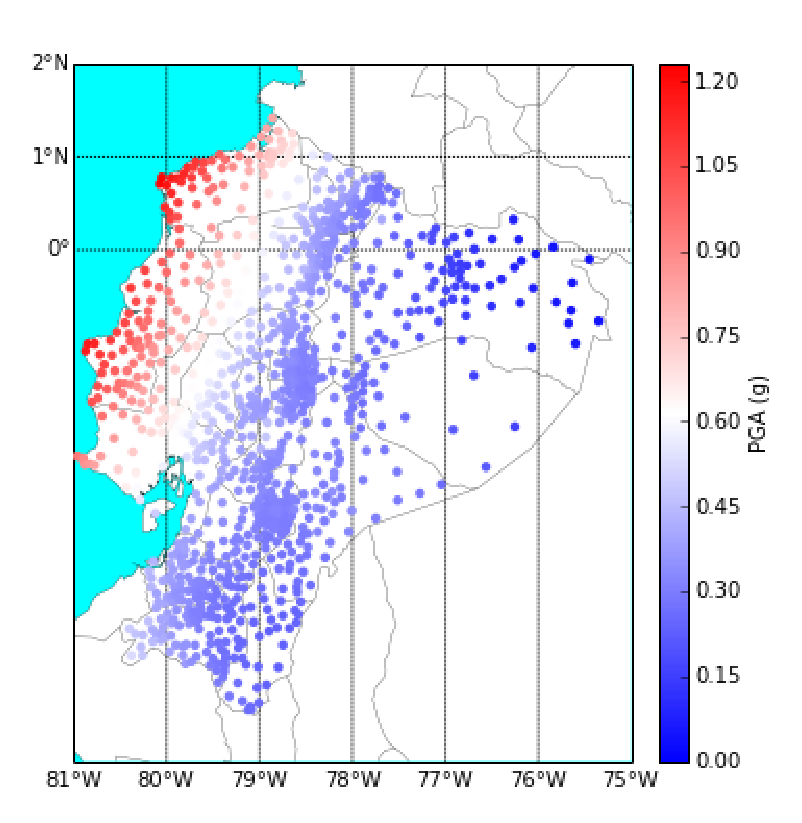
\includegraphics[width=7cm]{figures/hazard_Ecuador.eps}
  \caption{Seismic hazard map for a probability of exceedance of 10\% in 50 years.}
  \label{fig:hazard_map}
\end{figure}

\subsection{Plotting loss maps}
\label{subsec:plot-loss_maps}
A loss map provides the estimated losses for a collection of assets, for a certain return period (or probability of exceedance within a given interval of time). It is important to understand that these maps are not providing the distribution of losses for a seismic event or level of ground motion with the chosen return period, nor can the losses shown on the map be summed to obtain the corresponding aggregate loss with the same return period. This type of maps is simply providing the expected loss for a specified frequency of occurrence (or return period), for each asset.

To use this feature, it is necessary to define the path of the output file using the parameter \verb=loss_map_file=, as well as the exposure model used to perform the risk calculations through the parameter \verb=exposure_model=. Then, similarly to the method explained in section \ref{subsec:plot-collapse_maps} for collapse maps, it is possible to follow three approaches to generate the loss maps:\\

\begin{enumerate}
\item Aggregated loss map only.
\item Loss maps per vulnerability class only.
\item Both aggregated and vulnerability class-based.\\
\end{enumerate}

Then, there are a number of options that can be used to modify the style of the maps. These include the size of the marker of the map (\verb=marker_size=), the geographical limits of the map (\verb=bounding_box=), and the employment of a logarithmic spacing for the colour scheme (\verb=log_scale=). An example loss map for a single vulnerability class is presented in Figure \ref{fig:loss_map}.

\begin{figure}[htb]
  \centering
      \includegraphics[width=7cm]{figures/loss_map.png}
  \caption{Loss (economic) map for a probability of exceedance of 10\% in 50 years.}
  \label{fig:loss_map}
\end{figure}

As mentioned in the introductory section, it is also possible to convert any of the maps into a format (.csv) that is easily readable by GIS software. To do so, it is necessary to set the parameter \verb=export_map_to_csv= to \verb=True=. As an example, a map containing the average annual losses for Ecuador has been converted to the \verb=csv= format, and introduced into the QGIS software to produce the map presented in Figure \ref{fig:all_loss_map}.

\begin{figure}[htb]
  \centering
      \includegraphics[width=6cm]{figures/loss_map_AAL.png}
  \caption{Average annual (economic) losses for Ecuador.}
  \label{fig:all_loss_map}
\end{figure}


%----------------------------------------------------------------------------------------
%	CHAPTER 3
%----------------------------------------------------------------------------------------
% Risk part
\chapterimage{figures/chapter_head_2.pdf} % Chapter heading image
\include{book/chapter3/chapter3}

%----------------------------------------------------------------------------------------
%	CHAPTER 4
%----------------------------------------------------------------------------------------
% Vulnerability part
\chapterimage{figures/chapter_head_2.pdf} % Chapter heading image
\chapter{Vulnerability}
\label{chap:vulnerability}

    \section{Introduction}
    % Vulnerability functions, a fundamental component in the process of assessing seismic risk, can be defined as the probabilistic distribution of loss ratio conditional on a certain level of ground motion. Fragility functions, defining the probability of exceeding a set of damage states, can be combined with a consequence model, which establishes the relation between physical damage and a percentage of loss, to derive vulnerability functions. Building damage and repair cost data from past earthquakes can be used to derive both of these types of models [1–3]. However, empirical methodologies can have some disadvantages such as the subjectivity in allocating each building to a damage state or the lack of accuracy in the determination of the ground motion affecting the region. Furthermore, there are only a few dozen places in the world where post-earthquake damage and repair cost data has been collected from a number of buildings large enough to permit the development of reliable vulnerability functions. To overcome these limitations, analytical methodologies can be employed in either a single structure that is believed to be representative of a class of buildings, or a set of randomly generated buildings, modelled using structural analysis techniques, and subjected to specific lateral loading patterns or accelerograms.

% The various analytical methodologies for structural assessment can be categorized in two main groups: nonlinear dynamic analysis and nonlinear static analysis, each one having its own strengths and shortcomings. The main advantage in employing nonlinear dynamic analysis is certainly the fact that the actual dynamic phenomenon is reproduced by applying an acceleration time history at the base of the structure, leading in theory to more accurate results. However, the intrinsic modelling complexity (e.g., hysteric response models, equivalent viscous damping) combined with the heavy computational effort, is often impractical, thus favoring the employment of simpler methods, comprising nonlinear static analysis [13]. In this second approach, pushover curves are computed and used to estimate the maximum displacement response experienced by the structure for a given ground motion record. The main drawback of this simplified methodology lies with the assumption that the structural response obtained from horizontal static loading is representative of the one attained in the dynamic analysis.

% In this paper, several analytical methodologies are used to derive fragility functions for the same structural typology. A number of static approaches are investigated herein based on conventional and adaptive pushover analyses together with nonlinear static procedures (e.g., capacity spectrum method (CSM) [14], displacement coefficient method (DCM) [15], N2 method [16]), by using hundreds of ground motion records, to derive fragility functions for different levels of ground motion (intensity measure levels). Then, dynamic analysis is used as the baseline method in this sensitivity study, to yield conclusions regarding the relative accuracy of each method. Each set of fragility functions is transformed into vulnerability functions (i.e., probability of loss for a given level of ground motion) by calculating the mean damage ratio (i.e., ratio of cost of repair to cost of replacement) for a number of intensity measure levels

% The so-called NSP represent a simplified approach for the assessment of the seismic behavior of structures, included in guidelines such as the ATC-40 [14] and FEMA-440 [15] in the United States or the Eurocode 8 [43] in Europe. In this study, four distinct methodologies were employed: the CSM [14], the coefficient displacement method [15], the N2 method [16], and the adaptive CSM (ACSM) [44], which are further described in the following sections. These methodologies make use of capacity curves in terms of Sa versus Sd (i.e., the capacity of the equivalent SDOF). Each NSP is employed to estimate the target displacement obtained for each ground motion record, and this level of displacement is used to allocate the building in a damage state (according to the limit state criteria define in Section 2). This target displacement can be equated to the maximum roof displacement that would be experienced by the equivalent SDOF structure in a nonlinear dynamic analysis.

% Other NSPs such as the modal pushover analysis [45] or the adaptive modal combination procedure [46] have not yet been considered.

    \section{Definition input models}
    Capacity curves

Damage models

Ground motion records



	\section{Model generator}
	\label{sec:model-gen}
	To be completed by Vitor.
		
		\subsection{Generation of capacity curves using DBELA}
		\label{subsec:DBELA}
		The Displacement-based Earthquake Loss Assessment (DBELA) methodology permits the calculation of the displacement capacity of a collection of structures at a number of limit states (which could be structural or non-structural). These displacements are derived based on the capacity of an equivalent SDOF structure, following the principles of structural mechanics (\cite{CrowleyEtAl2004}; \cite{BalEtAl2010}; \cite{SilvaEtAl2013}).\\
The displacement at the height of the centre of seismic force of the original structure ($H_{CSF}$) can be estimated by multiplying the base rotation by the height of the equivalent SDOF structure ($H_{SDOF}$), which is obtained by multiplying the total height of the actual structure ($H_T$) by an effective height ratio ($ef_h$), as illustrated in Figure \ref{fig:efh}:

\begin{figure}[htb]
  \centering
      \includegraphics[width=8cm]{Figures/effective_height.png}
  \caption{Definition of effective height coefficient \cite{GlaisterPinho2003}.}
  \label{fig:efh}
\end{figure}
 
\cite{PinhoEtAl2002} and \cite{GlaisterPinho2003} proposed formulae for estimating the effective height coefficient for different response mechanisms. For what concerns the beam sway mechanism (or distributed plasticity mechanism, as shown in Figure \ref{fig:mechanisms}), a ratio of 0.64 is proposed for structures with 4 or less storeys, and 0.44 for structures with 20 or more storeys. For any structures that might fall within these limits, linear interpolation should be employed. With regards to the column-sway mechanism (or concentrated plasticity mechanism, as shown in Figure \ref{fig:mechanisms}), the deformed shapes vary from a linear profile (pre-yield) to a non-linear profile (post-yield). As described in \cite{GlaisterPinho2003}, a coefficient of 0.67 is assumed for the pre-yield response and the following simplified formula can be applied post-yield (to attempt to account for the ductility dependence of the effective height post-yield coefficient):
 
\begin{equation}
ef_h = 0.67 - 0.17\frac{\epsilon_{s(LS_i)}-\epsilon_y}{\epsilon_{s(LS_i)}}
\end{equation}
 
\begin{figure}[htb]
  \centering
      \includegraphics[width=10cm]{Figures/collapse_mechanisms.png}
  \caption{Deformed profiles for beam-sway (left) and column-sway (right) mechanisms\cite{PaulayPriestley2002}.}
  \label{fig:mechanisms}
\end{figure}
The displacement capacity at different limit states (either at yield ($\delta_y$) or post-yield ($\delta_{(LSi)}$) for bare frame or infilled reinforced concrete structures can be computed using simplified formulae, which are distinct if the structure is expected to exhibit a beam- or column-sway failure mechanism. These formulae can be found in \cite{BalEtAl2010} or \cite{SilvaEtAl2013}, and their mathematical formulation is described in detail in \cite{CrowleyEtAl2004}.\\

In order to estimate whether a given frame will respond with a beam- or a column-sway mechanism it is necessary to evaluate the properties of the storey. A deformation-based index ($R$) has been proposed by \cite{AboElEzz2008} which reflects the relation between the stiffness of the beams and columns. This index can be computed using the following formula:
\begin{equation}
R = \frac{^{h_b}/_{l_b}}{^{h_c}/_{l_c}}
\end{equation}

Where $l_c$ stands for the column length. \cite{AboElEzz2008} proposed some limits for this index applicable to bare and fully infilled frame structures, as described in Table \ref{table:AboElEzz2008}.
\begin {table}[htb]
\caption{Limits for the deformation-based sway index proposed by \cite{AboElEzz2008}} 
\label{table:AboElEzz2008} 
\begin{center}
  \begin{tabular}{ | c | c | c |}
  \hline
    Building Typology & Beam sway & Column sway  \\ \hline
    Bare frames & R$\leq$1.0 & R>1.5 \\ \hline
    Fully infilled frames & R$\leq$1.0 & R>1.0 \\ \hline
  \end{tabular}
\end{center}
\end{table}

The calculation of the corresponding spectral aceleration is performed by assuming a perfectly elasto-plastic behaviour. Thus, the spectral displacement for the yeilding point is used to derive the associated acceleration through the following formula:

\begin{equation}
Sa_i = \frac{4\pi^2Sd_i}{T_y^2}
\end{equation}

Where $T_y$ stands for the yielding period which can be calculated using simplified formulae (e.g. \cite{CrowleyPinho2004}; \cite{CrowleyPinho2006}), as further explained in Section \ref{subsec:DBELA_Silva2013}. Due to the assumption of the elasto-plastic behaviour, the spectral acceleration for the remaining limit states (or spectral displacemens) will be the same (see Figure \ref{fig:DBELA_cc}). \\ 

In order to use this methodology it is necessary to define a building model, which specifies the probabilistic distribution of the geometrical and material properties. This information is currently stored in a $csv$ file (tabular format), as presented in Table \ref{table:building_model}.
 
\begin {table}[htb]
\caption{Example of a building model compatible with the DBELA method.} 
\label{table:building_model} 
\begin{center}
  \begin{tabular}{ | l | l | l | l | l | l |}
  \hline
Structure type & bare frame &  &  &  &  \\ \hline
ductility & ductile &  &  &  &  \\ \hline
number of storeys & 3 &  &  &  &  \\ \hline
steel modulus & lognormal & 210000 & 0.01 & 0 & inf \\ \hline
steel yield strength & normal & 371.33 & 0.24 & 0 & inf \\ \hline
ground floor height & discrete & 2.8 3.1 3.2 & 0.48 0.15 0.37 & 0 & inf \\ \hline
regular floor height & lognormal & 2.84 & 0.08 & 0 & inf \\ \hline
column depth & lognormal & 0.45 & 0.12 & 0.3 & 0.6 \\ \hline
beam length & gamma & 3.37 & 0.38 & 0 & inf \\ \hline
beam depth & lognormal & 0.6 & 0.16 & 0.4 & 0.8 \\ \hline
  \end{tabular}
\end{center}
\end{table}

The \verb=structure type= can be set to \verb=bare frame= or \verb=infilled frame=, while the parameter \verb=ductility= can be equal to \verb=ductile= or \verb=non-ductile=. The variable \verb=number of storeys= must be equal to an integer defining the number of floors of the building class. The following parameters (\verb=steel modulus= , \verb=steel yield strength= , \verb=ground floor height= , \verb=regular floor height= , \verb=column depth= , \verb=beam length= , \verb=beam depth=) define the represent the geometrical and material properties of the building class, and can defined in a probabilitic manner. Currently, three parametric statistical models have been implemented (\verb=normal= , \verb=lognormal= and \verb=gamma=), as well as discrete (i.e. probability mass function) model (\verb=discrete=). The model that should be used must be specified on the second column. Then, for the former type of models (parametric), the mean and coefficient of variation should be provided in the third and forth columns, respectively. For the discrete model, the central values of the bins and corresponding probabilities of occurance should be defined in the third and forth columns, respectively. The last two columns can be used to truncate the probabilistic distribution between a minimum (fifth column) and maximum (sixth column) values. In order to define a parameter in a deterministic manner (no variability), the coeficient of variation for the associated attribute can be set to zero, and the same value (mean) will be used repeatedly.\\

The location of the building model and the damage model (see Section \ref{subsec:dmg_model}) should be specified in the variables \verb=building_model= and the \verb=damage_model=, respectively. The number of capacity curves that should be generated must be defined using the parameter \verb=no_assets=. Then, after importing the module \verb=DBELA=, the set of capacity curves can be generated using the following commands:

\begin{Verbatim}[frame=single, commandchars=\\\{\}, samepage=true]
building_class_model = DBELA.read_building_class_model(building_model)
assets = DBELA.generate_assets(building_class_model,no_assets)
capacity_curves = DBELA.generate_capacity_curves(assets,damage_model)
\end{Verbatim}

The first function (\verb=read_building_class_model=) processes the information about the building class; the second function (\verb=generate_assets=) uses a Monte Carlo sampling process to generate a set of synthetic structural models (each one with unique geometrical and material properties); and the final function (\verb=generate_capacity_curves=) combines the generated assets with the damage model to calculate a capacity curve per structure. Figure \ref{fig:DBELA_cc} presents a collection of capacity curves generated using this methodology.

\begin{figure}[htb]
  \centering
      \includegraphics[width=8cm]{Figures/synthethic_capacity_curves.png}
  \caption{Capacity curves for reinforced concrete bare frames generated using the DBELA methodology.}
  \label{fig:DBELA_cc}
\end{figure}
		
		\subsection{Generation of capacity curves using SP-BELA}
		\label{subsec:DBELA}
		The Displacement-based Earthquake Loss Assessment (DBELA) methodology permits the calculation of the displacement capacity of a collection of structures at a number of limit states (which could be structural or non-structural). These displacements are derived based on the capacity of an equivalent SDOF structure, following the principles of structural mechanics (\cite{CrowleyEtAl2004}; \cite{BalEtAl2010}; \cite{SilvaEtAl2013}).\\
The displacement at the height of the centre of seismic force of the original structure ($H_{CSF}$) can be estimated by multiplying the base rotation by the height of the equivalent SDOF structure ($H_{SDOF}$), which is obtained by multiplying the total height of the actual structure ($H_T$) by an effective height ratio ($ef_h$), as illustrated in Figure \ref{fig:efh}:

\begin{figure}[htb]
  \centering
      \includegraphics[width=8cm]{Figures/effective_height.png}
  \caption{Definition of effective height coefficient \cite{GlaisterPinho2003}.}
  \label{fig:efh}
\end{figure}
 
\cite{PinhoEtAl2002} and \cite{GlaisterPinho2003} proposed formulae for estimating the effective height coefficient for different response mechanisms. For what concerns the beam sway mechanism (or distributed plasticity mechanism, as shown in Figure \ref{fig:mechanisms}), a ratio of 0.64 is proposed for structures with 4 or less storeys, and 0.44 for structures with 20 or more storeys. For any structures that might fall within these limits, linear interpolation should be employed. With regards to the column-sway mechanism (or concentrated plasticity mechanism, as shown in Figure \ref{fig:mechanisms}), the deformed shapes vary from a linear profile (pre-yield) to a non-linear profile (post-yield). As described in \cite{GlaisterPinho2003}, a coefficient of 0.67 is assumed for the pre-yield response and the following simplified formula can be applied post-yield (to attempt to account for the ductility dependence of the effective height post-yield coefficient):
 
\begin{equation}
ef_h = 0.67 - 0.17\frac{\epsilon_{s(LS_i)}-\epsilon_y}{\epsilon_{s(LS_i)}}
\end{equation}
 
\begin{figure}[htb]
  \centering
      \includegraphics[width=10cm]{Figures/collapse_mechanisms.png}
  \caption{Deformed profiles for beam-sway (left) and column-sway (right) mechanisms\cite{PaulayPriestley2002}.}
  \label{fig:mechanisms}
\end{figure}
The displacement capacity at different limit states (either at yield ($\delta_y$) or post-yield ($\delta_{(LSi)}$) for bare frame or infilled reinforced concrete structures can be computed using simplified formulae, which are distinct if the structure is expected to exhibit a beam- or column-sway failure mechanism. These formulae can be found in \cite{BalEtAl2010} or \cite{SilvaEtAl2013}, and their mathematical formulation is described in detail in \cite{CrowleyEtAl2004}.\\

In order to estimate whether a given frame will respond with a beam- or a column-sway mechanism it is necessary to evaluate the properties of the storey. A deformation-based index ($R$) has been proposed by \cite{AboElEzz2008} which reflects the relation between the stiffness of the beams and columns. This index can be computed using the following formula:
\begin{equation}
R = \frac{^{h_b}/_{l_b}}{^{h_c}/_{l_c}}
\end{equation}

Where $l_c$ stands for the column length. \cite{AboElEzz2008} proposed some limits for this index applicable to bare and fully infilled frame structures, as described in Table \ref{table:AboElEzz2008}.
\begin {table}[htb]
\caption{Limits for the deformation-based sway index proposed by \cite{AboElEzz2008}} 
\label{table:AboElEzz2008} 
\begin{center}
  \begin{tabular}{ | c | c | c |}
  \hline
    Building Typology & Beam sway & Column sway  \\ \hline
    Bare frames & R$\leq$1.0 & R>1.5 \\ \hline
    Fully infilled frames & R$\leq$1.0 & R>1.0 \\ \hline
  \end{tabular}
\end{center}
\end{table}

The calculation of the corresponding spectral aceleration is performed by assuming a perfectly elasto-plastic behaviour. Thus, the spectral displacement for the yeilding point is used to derive the associated acceleration through the following formula:

\begin{equation}
Sa_i = \frac{4\pi^2Sd_i}{T_y^2}
\end{equation}

Where $T_y$ stands for the yielding period which can be calculated using simplified formulae (e.g. \cite{CrowleyPinho2004}; \cite{CrowleyPinho2006}), as further explained in Section \ref{subsec:DBELA_Silva2013}. Due to the assumption of the elasto-plastic behaviour, the spectral acceleration for the remaining limit states (or spectral displacemens) will be the same (see Figure \ref{fig:DBELA_cc}). \\ 

In order to use this methodology it is necessary to define a building model, which specifies the probabilistic distribution of the geometrical and material properties. This information is currently stored in a $csv$ file (tabular format), as presented in Table \ref{table:building_model}.
 
\begin {table}[htb]
\caption{Example of a building model compatible with the DBELA method.} 
\label{table:building_model} 
\begin{center}
  \begin{tabular}{ | l | l | l | l | l | l |}
  \hline
Structure type & bare frame &  &  &  &  \\ \hline
ductility & ductile &  &  &  &  \\ \hline
number of storeys & 3 &  &  &  &  \\ \hline
steel modulus & lognormal & 210000 & 0.01 & 0 & inf \\ \hline
steel yield strength & normal & 371.33 & 0.24 & 0 & inf \\ \hline
ground floor height & discrete & 2.8 3.1 3.2 & 0.48 0.15 0.37 & 0 & inf \\ \hline
regular floor height & lognormal & 2.84 & 0.08 & 0 & inf \\ \hline
column depth & lognormal & 0.45 & 0.12 & 0.3 & 0.6 \\ \hline
beam length & gamma & 3.37 & 0.38 & 0 & inf \\ \hline
beam depth & lognormal & 0.6 & 0.16 & 0.4 & 0.8 \\ \hline
  \end{tabular}
\end{center}
\end{table}

The \verb=structure type= can be set to \verb=bare frame= or \verb=infilled frame=, while the parameter \verb=ductility= can be equal to \verb=ductile= or \verb=non-ductile=. The variable \verb=number of storeys= must be equal to an integer defining the number of floors of the building class. The following parameters (\verb=steel modulus= , \verb=steel yield strength= , \verb=ground floor height= , \verb=regular floor height= , \verb=column depth= , \verb=beam length= , \verb=beam depth=) define the represent the geometrical and material properties of the building class, and can defined in a probabilitic manner. Currently, three parametric statistical models have been implemented (\verb=normal= , \verb=lognormal= and \verb=gamma=), as well as discrete (i.e. probability mass function) model (\verb=discrete=). The model that should be used must be specified on the second column. Then, for the former type of models (parametric), the mean and coefficient of variation should be provided in the third and forth columns, respectively. For the discrete model, the central values of the bins and corresponding probabilities of occurance should be defined in the third and forth columns, respectively. The last two columns can be used to truncate the probabilistic distribution between a minimum (fifth column) and maximum (sixth column) values. In order to define a parameter in a deterministic manner (no variability), the coeficient of variation for the associated attribute can be set to zero, and the same value (mean) will be used repeatedly.\\

The location of the building model and the damage model (see Section \ref{subsec:dmg_model}) should be specified in the variables \verb=building_model= and the \verb=damage_model=, respectively. The number of capacity curves that should be generated must be defined using the parameter \verb=no_assets=. Then, after importing the module \verb=DBELA=, the set of capacity curves can be generated using the following commands:

\begin{Verbatim}[frame=single, commandchars=\\\{\}, samepage=true]
building_class_model = DBELA.read_building_class_model(building_model)
assets = DBELA.generate_assets(building_class_model,no_assets)
capacity_curves = DBELA.generate_capacity_curves(assets,damage_model)
\end{Verbatim}

The first function (\verb=read_building_class_model=) processes the information about the building class; the second function (\verb=generate_assets=) uses a Monte Carlo sampling process to generate a set of synthetic structural models (each one with unique geometrical and material properties); and the final function (\verb=generate_capacity_curves=) combines the generated assets with the damage model to calculate a capacity curve per structure. Figure \ref{fig:DBELA_cc} presents a collection of capacity curves generated using this methodology.

\begin{figure}[htb]
  \centering
      \includegraphics[width=8cm]{Figures/synthethic_capacity_curves.png}
  \caption{Capacity curves for reinforced concrete bare frames generated using the DBELA methodology.}
  \label{fig:DBELA_cc}
\end{figure}
		
		\subsection{Generation of capacity curves using point dispersion}
		\label{subsec:dispersion}
		This module of the Risk Modeller's Toolkit allows the generation of a large number of capacity curves, based on a single median curve, and information regarding the expected dispersion at each point of the curve. \\

As an example, in a study carried out by \cite{SilvaEtAl2014b}, several capacity curves were derived for 100 reinforced concrete frames with 4 storeys without seismic provisions, as illustrated in Figure \ref{fig:set_cc}. In addition to the mean and median capacity curves, an additional capacity curve was also derived using the mean geometrical and material properties of the building class of interest. From this distribution of curves, it is possible to assess the probabilistic distribution of a number of specific points, such as the yielding or ultimate capacities. Then, once adequate statistical models have been defined for these specific points, it is possible to reproduce the the distribution of capacity curves using a Monte Carlo approach. If one assumes that such distribution could be applicable to other building classes, then it is possible to produce sets of capacity curves (as a way to propagate the building-to-building variability), based on this dispersion and a capacity curve believed to be representative of the median capacity of the building class.

\begin{figure}[htb]
  \centering
      \includegraphics[width=7cm]{figures/set_capacity_curves.png}
  \caption{Capacity curves using a displacement-based adaptive pushover approach \citep{SilvaEtAl2014b}.}
  \label{fig:set_cc}
\end{figure}

To use this methodology, it is necessary to import the module \verb=point_dispersion=. Then, the spectral acceleration and displacement of the median capacity curve should be defined in the vectors \verb=Sa= and \verb=Sd=, respectively. For each point in these vectors, it is necessary to provide the corresponding variability (as a form of a coefficient of variation), in the variables \verb=Sa_cov= and \verb=Sd_cov=. The type of probabilistic distribution that should be used must be defined using the parameter \verb=type_of_dist=. Currently this module allows \verb=normal= and \verb=lognormal=. An example of the definition of these variables is provided below. In this case, the capacity curves are being defined using three points (the yielding capacity, the point of maximum force and the ultimate displacement).

\begin{Verbatim}[frame=single, commandchars=\\\{\}, samepage=true]
Sa = [0.25, 0.45, 0.35]
Sa_cov = [0.25, 0.30, 0.30]
Sd =  [0.10, 0.20, 0.50]
Sd_cov = [0.20, 0.30, 0.45]
type_dist = 'normal'
\end{Verbatim}

Within this methodology, it is also possible to specify the correlation in the spectral acceleration (\verb=Sa_corr=) and spectral displacement (\verb=Sd_corr=). If these correlation factors are set to zero, then the sampling process is carried out independently. On the other hand, if these parameters are set to one, then a full correlation is assumed, which means, for example, if a higher displacement is sampled for the yielding point, then a large displacement will also be sampled for the remaining points. Values between zero and one will lead to intermediate situations. It is also possible to control the correlation between the spectral acceleration and displacement, using the variable \verb=SaSd_corr=.
The dispersion of the synthetic capacity curves can also be controlled through the allowed number of standard deviations above or below the median capacity curve. This aspect is controlled by the parameter \verb=truncation=, which should be equal to the maximum number of allowed standard deviations. for example, a value equal to 1 signifies that all of the generated capacity curves will be within one standard deviation of the median capacity curve. Finally, the number of capacity curves that will be generated needs to be specified using the variable \verb=no_cc=. Figure \ref{fig:dispersion_cc} illustrates 100 capacity curves generated using the data provided above.

\begin{figure}[htb]
  \centering
      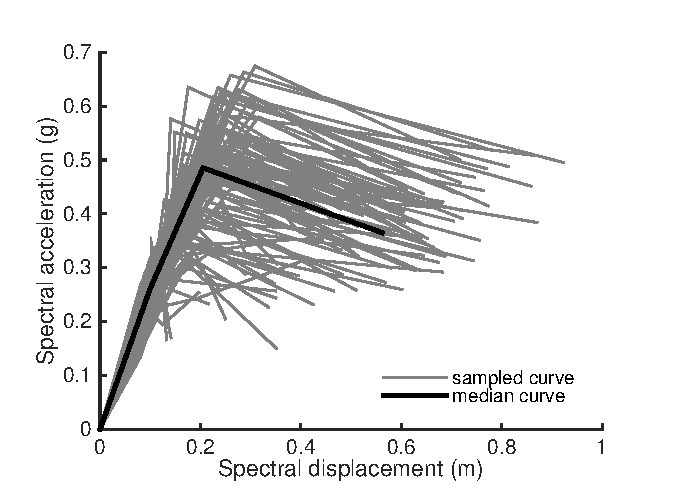
\includegraphics[width=8cm]{figures/dispersion_cc.eps}
  \caption{Capacity curves generated using the point dispersion approach.}
  \label{fig:dispersion_cc}
\end{figure}
			
	\section{Conversion from MDOF to SDOF}
	\label{sec:mdof_to_sdof}
	This feature of the Risk Modeller's Toolkit enables the user to derive equivalent single-degree-of-freedom (SDOF) capacity curves for multiple-degree-of-freedom (MDOF) structures. Several structural analysis packages allow the user to perform a reliable pushover analysis on a nonlinear model of the MDOF structure. The results of the pushover analysis (in terms of a pushover curve) can be provided as input to one of the methods in this module. This module allows the conversion of the MDOF results into 'equivalent SDOF' results, thus making them compatible with a wide range of non-linear static procedures. At present, two methods are provided in this module for obtaining equivalent SDOF capacity curves for an MDOF system.

A pushover curve is generated by subjecting a detailed or a carefully simplified structural model to one or more lateral load patterns and then increasing the magnitude of the total load to generate a nonlinear inelastic force-deformation relationship. The load vector is usually a representation of the load acting on the structure vibrating in its first mode .In ATC-40 Procedure A , the global parameters used are spectral acceleration and spectral displacement. Therefore a Capacity curve used in this procedure is a curve obtained by transforming the structure base shear vs. roof displacement curve into an Equivalent Single Degree of Freedom structure, acceleration vs. displacement curve .The equivalent SDOF properties correspond to the first mode properties of the detailed structure .In this chapter equations needed to convert the pushover curve into a capacity curve will be developed.
	
		\subsection{Conversion based on one mode of vibration}
		\label{subsec:one_mode}
		This method allows the user to convert a pushover curve for an MDOF system into an equivalent SDOF capacity curve, considering the first mode of vibration only. The supplied pushover curve, which is in terms of base shear and roof displacement, is transformed into an equivalent SDOF capacity curve, which is in terms of spectral acceleration and spectral displacement. The properties of the equivalent SDOF model correspond to the properties of the first mode of vibration of the MDOF system. The roof displacement is converted to $S_d$ by normalising by the participation factor of the first mode of vibration, whereas the base shear is normalised to give $S_a$ using the the participation factor and modal mass for the first mode. Details of this conversion method can be found in \citet{ATC1996}, \citet{FEMA4402005}, and Eurocode 8 \citep{CEN2005}.

The equivalent system acceleration $S_{a-capacity}$ and displacement $S_{d-capacity}$ are calculated as:
\begin{equation}
	S_{a-capacity} = \frac{V_{b-pushover}}{M_{1}^{*} g}
\end{equation}

\begin{equation}
	S_{d-capacity} = \frac{\Delta_{roof}}{\Gamma_{1} \phi_{1, roof}}
\end{equation}

where 􏰁$\Gamma_{1}$ and $M_{1}^{*}$ are the modal participation factor and the modal mass of the first mode respectively, $\Delta_{roof}$ is the displacement of the roof, $\phi_{1, roof}$ is the roof displacement in the first mode, and $V_{b-pushover}$ is the total base shear from the pushover analysis.
		
		\subsection{Conversion using an adaptive approach}
		\label{subsec:adaptive}
		Adaptive pushover methods have the advantage of better accounting for stiffness degradation, influence of higher mode effects, and spectral amplifications because of ground motion frequency content. In this method, instead of applying an invariant load vector, the structural properties of the model are evaluated at each step of the analysis, and the loading pattern is updated accordingly. In this way, the variation in the structural stiffness at different deformation levels, and consequently the system degradation and period elongation can be accounted for. The only apparent drawback of this methodology can be the additional computation time required to assess the structural characteristics at every step.

The equivalent system displacement $\Delta_{sys,k}$ at step $k$ is calculated as:
\begin{equation}
	\Delta_{sys,k} = \frac{\sideset{}{_i}\sum m_i \Delta_{i,k}^2}{\sideset{}{_i}\sum m_i \Delta_{i,k}}
\end{equation}
Note that $\Delta_{sys,k}$ is defined to be the inverse of the modal participation factor.

The equivalent system acceleration $\S_{a-cap,k}$ at step $k$ is calculated as:
\begin{equation}
	S_{a-cap,k} = \frac{V_{b,k}}{M_{sys,k} g}
\end{equation}

The equivalent system mass $M_{sys,k}$ is defined as:
\begin{equation}
	M_{sys,k} = \frac{\sideset{}{_i}\sum m_i \Delta_{i,k}}{M_{sys,k} g}
\end{equation}
Note that $M_{sys,k}$ is the modal mass of the system at analysis step $k$.
		
	\section{Derivation of fragility}
	\label{sec:derivation_fragility}
	As explained by Lin and Miranda (2008), performance-based evaluation of structures requires the estimation of a demand spectrum that can properly take into account the inelastic behaviour of the structure(s) under analysis, namely, their capacity to dissipate seismic energy through hysteresis (Monteiro, 2011). In order to achieve this, two main approaches exist. The first one estimates the maximum inelastic deformation of a structure by applying a modification factor to its maximum linear elastic deformation. This factor can be damping-based or ductility-based. The former case reduces both the displacement and acceleration spectral coordinates by a reduction factor B, which is based on the equivalent viscous damping of the system. On the other hand, the latter reduce the spectral acceleration ordinates of a 5\%-damped elastic response spectrum by a factor dependant on the ductility of the system.  

The second approach estimates the maximum deformation of a nonlinear structure as the maximum deformation of an equivalent linear system with longer period of vibration (i.e. more flexible lateral stiffness) and higher viscous damping than those of the “original” structure. These parameters can be dependant either on the displacement ductility of the system (which implies an iterative process) or on the strength ratio R (or strength reduction factor). 
			
		\subsection{SPO2IDA (Vamvatsikos and Cornell 2006)}
		\label{subsec:SPO2IDA}
		The tool spo2ida (Vamvatsikos and Cornell, 2006) is capable of converting static pushover curves into 16\%, 50\% and 84\% ida curves, as shown in Figure~\ref{fig:spo2ida}, using empirical relationships from a large database of incremental dynamic analysis results. 

\begin{figure}[!htbp]
\centering
\includegraphics[width=10cm]{./figures/spo2ida.jpg}
\caption{spo2ida tool: IDA curves derived from Pushover curve.}
\label{fig:spo2ida}
\end{figure}

The spo2ida tool is applicable to any kind of multi-linear capacity curve. Making use of this tool is is possible to estimate single building fragility curve and fragility curves derived for single buildings can be combined in a unique fragility curve, which considers also the inter-building uncertainty.\\

Given an idealised capacity curve the spo2ida tool uses an implicit R-$\mu$-T relation to correlate nonlinear displacement, expressed in terms of ductility $\mu$ to the corresponding median capacities in terms of the parameters R. R is the lateral strength ratio, defined as the ratio between the spectral acceleration S$_a$ and the yielding capacity of the system S$_{ay}$. Each branch of the capacity curve, hardening, softening and residual plateau, is converted to a corresponding branch of the three ida curves, using the R-$\mu$-T relation, which is a function of the hardening stiffness, the softening stiffness and the residual force. These parameters are derived from the idealised pushover capacity expressed in $\mu$-R terms, as well as the ductility levels at the onset of each branch. If some of the branches of the pushover curve are missing because of the seismic behaviour of the system, spo2ida can equally work with bilinear, trilinear and quadrilinear idealisations.\\

The result of the spo2ida routine is thus a list of ductility levels and corresponding R values at 50\%, 16\% and 84\% percentiles. For any inelastic displacement, and therefore any level of ductility $\mu$ the corresponding $R_{50\%}$, $R_{16\%}$, and $R_{84\%}$ values are found interpolating the aforementioned ida curves.
Median R and its dispersion at ductility levels corresponding to the damage thresholds ds can thus be determined, and converted into median $S_{a, ds}$ and its dispersion due to record-to-record variability $\beta_{S_{a d}}$ according to equations \ref{eq:SaR} and \ref{eq:betaR}. 

\begin{equation}
\hat{S}_{a, ds} = R_{50\%}(\mu_{ds}) S_{ay}
\label{eq:SaR}
\end{equation}
\begin{equation}
\beta_{S_{a d}} = \beta_{R(\mu_{ds})} = \frac{\ln R(\mu_{ds})_{84\%} - \ln R(\mu_{ds})_{16\%}}{2}
\label{eq:betaR}
\end{equation} 

If dispersion due to uncertainty in the limit state definition $\beta_{\theta c}$ is different from zero a Monte Carlo sampling needs to be performed to combine it with the record-to-record dispersion. Different values of ductility limit state are sampled from the  lognormal distribution with median the median value of the ductility limit state, and dispersion the input $\beta_{\theta c}$. For each of these ductilities the corresponding median $R_{50\%}$ and R$_{16\%}$, R$_{84\%}$ are found and converted into $\hat{S}_{a,ds}$ and $\beta_S_{a d}$ according to equation \ref{eq:SaR} and \ref{eq:betaR}. MC random S$_a$ for each MC sampled ductility limit state are computed, and their median and the dispersion are estimated. These parameters constitute the median $\hat{S}_{a,ds}$ and the total dispersion $\beta_{S_a}$ for the considered damage state. The procedure is repeated for each damage state.

\subsubsection{Multiple-Building Fragility and Vulnerability function}
\label{subsubsec:multiple-buildings}
If multiple buildings have been input to derive fragility function for a class of buildings all $\hat{S}_{a, blg}$ and $\beta_{S_a, blg}$ are combined in a single lognormal curve. A minimum of 5 buildings should be considered to obtain reliable results for the class.\\ 
A new issue arises when multiple buildings are considered: the S$_a$ at the fundamental period of each building should be converted to a common intensity measure, to be able to combine the different fragility functions. A common intensity measure is selected to be S$_a$ at the period T$_{av}$, which is a weighted average of the individual building fundamental periods T$_1$. Then each individual fragility needs to be expressed in terms of the common S$_a$(T$_{av}$), using a spectrum. FEMA P-695 far field set of 44 accelerograms (22 records for the two directions) was used to derive a mean uniform hazard spectrum, and the ratio between the S$_a$ at different periods is used to scale the fragility functions. It can be noted that the actual values of the spectrum are not important, but just the spectral shape. 
The median $\hat{S}_a$ is converted to the mean $\mu_{ln(S_a)}$ of the corresponding normal distribution ($\mu_{ln(S_a)} = ln(\hat{S}_a)$) and simply scaled to the common intensity measure as follows:

\begin{equation}
\mu_{ln(S_a), blg} = \mu_{ln(S_a), blg} S(T_{av})/ S(T_{1, blg})
\end{equation}
\begin{equation}
\beta_{S_a, blg} = \beta_{S_a, blg} S(T_{av})/ S(T_{1, blg})
\label{eq:Sa(Tav)}
\end{equation}

where $S(T_{av})/ S(T_{1, blg}$ is defined as spectral ratio. Finally the parameters of the single lognormal curve for the class of buildings, mean and dispersion, can be computed as the weighted mean of the single means and the weighted SRSS of the inter-building and intra-building standard deviation, the standard deviation of the single means and the single dispersions respectively, as shown in the following equations:

\begin{equation}
\mu_{ln(S_a), tot} = \sum_{i=0}^{n.blg} w_{blg-i} \mu_{ln(S_a), blg-i}
\label{eq:combination-lognormals-mu}
\end{equation}
\begin{equation}
\beta_{S_a, tot} = \sqrt{ \sum_{i=0}^{n.blg} w_{blg-i} ((\mu_{ln(S_a), blg-i}-\mu_{ln(S_a), tot})^2+ \beta_{S_a, blg-i}^2})
\label{eq:combination-lognormals-sigma}
\end{equation}

In order to use this methodology, it is necessary to load one or multiple capacity curves as described in Section \ref{subsec:cap_curves}. It is also necessary to specify the type of shape the capacity curves want to be idealised with, using the parameter \verb=idealised_type= (either \verb=bilinear= or \verb=quadrilinear=). If the user has already at disposal an idealised multilinear pushover curve for each building, the variable \verb=Idealised= in the csv input file should be set to \verb=TRUE=, and idealised curves should be provided according to what described in section \ref{subsec:cap_curves}. Then, it is necessary to specify a damage model using the parameter \verb=damage_model= (see Section \ref{subsec:dmg_model}).

If dispersion due to uncertainty in the limit state definition is different from zero a Monte Carlo sampling needs to be performed to combine it with the record-to-record dispersion. The number of Monte Carlo samples should be defined in the variable \verb=montecarlo_samples=.
After importing the module \verb=SPO2IDA_procedure=, it is possible to calculate the parameter of the fragility model, median and dispersion, using the following command:

\begin{Verbatim}[frame=single, commandchars=\\\{\}, samepage=true]
fragility_model = SPO2IDA_procedure.calculate_fragility(capacity_curves,
... idealised_capacity, damage_model, montecarlo_samples, Sa_ratios,
... ida_plotflag)
\end{Verbatim}

where \verb=Sa_ratios= is the spectral ratio variable needed to combine together fragility curves for many buildings, as described in Section \ref{subsec:derive_fragility}, and \verb=ida_plotflag= indicates whether ida plots want to be displayed (\verb=ida_plotflag= = 1) or not (\verb=ida_plotflag= = 0).
		
		\subsection{Dolsek and Fajfar 2004}
		\label{subsec:DolsekFajfar}
		To be completed by Chiara.

		\subsection{Ruiz Garcia and Miranda 2007}
		\label{subsec:RuizGarciaMiranda}
		\input{book/chapter4/derivation_fragility/Ruiz_Garcia_Miranda_2007}
		
		\subsection{Vidic and Fajfar 1994}
		\label{subsec: VidicFajfar1994}
		\input{book/chapter4/derivation_fragility/Vidic_Fajfar_1994}
		
		\subsection{Lin and Miranda 2008}
		\label{subsec:LinMiranda}
		This methodology estimates the maximum inelastic displacement of an existing structure based on the maximum elastic displacement response of its equivalent linear system without the need for iterations, based on the strength ratio R (instead of the most commonly used ductility ratio).\\
In order to evaluate an existing structure, a pushover analysis should be conducted in order to obtain the capacity curve. This curve should be bilinearised in order to obtain the yield strength, fy, the postyield stiffness ratio, $\alpha$, and the strength ratio, R. With these parameters, along with the initial period of the system, it is possible to estimate the optimal period shift (i.e. the ratio between the period of the equivalent linear system and the initial period) and the equivalent viscous damping, $\xi$eq, of the equivalent linear system, using the following relationships derived by \citep{LinMiranda2008}.
	 
\begin{equation}
\frac{T_{eq}}{T_{0}} = 1 + \frac{m_1}{T_0^{m_2}}\left(R^{1.8}-1\right)
\end{equation} 

\begin{equation}
\xi_{eq} = \xi_{0} + \frac{n_1}{T_0^{n_2}}\left(R-1\right)
\end{equation}   

Where the coefficients m1, m2, n1, and n2 depend on the postyield stiffness ratio, as shown in the following Table \ref{table:LinMiranda2008}.

\begin {table}[htb]
\caption{Paramereters for the estimation of the reduction factor C proposed by \citep{LinMiranda2008}} 
\label{table:LinMiranda2008} 
\begin{center}
  \begin{tabular}{ | c | c | c | c | c |}
    \hline
    $\alpha$ & $m_1$ & $m_2$ & $n_1$ & $n_2$ \\ \hline
    0\% & 0.026 & 0.87 & 0.016 & 0.84 \\ \hline
    5\% & 0.026 & 0.65 & 0.027 & 0.55 \\ \hline
    10\% & 0.027 & 0.51 & 0.031 & 0.39 \\ \hline
    20\% & 0.027 & 0.36 & 0.030 & 0.24 \\ \hline
  \end{tabular}
\end{center}
\end{table}
Using $\xi$eq and the damping modification factor, B (as defined in Table 15.6-1 of NEHRP-2003), it is possible to construct the reduced displacement spectrum, Sd(T, $\xi$eq) from which the maximum displacement demand (i.e. the displacement corresponding to the equivalent system period) can be obtained, using the following equation:
	  
In order to use this methodology, it is necessary to load one or multiple capacity curves as described in Section \ref{subsec:cap_curves}, as well as a set of ground motion records as explained in Section \ref{subsec:gmrs}. Then, it is necessary to specify a damage model using the parameter \verb=damage_model= (see Section \ref{subsec:dmg_model}). After importing the module \verb=lin_miranda_2008=, it is possible to calculate the distribution of structures across the set of damage state for each ground motion record using the following command:

\begin{Verbatim}[frame=single, commandchars=\\\{\}, samepage=true]
PDM, Sds = lin_miranda_2008.calculate_fragility(capacity_curves,gmrs,...
damage_model,damping)
\end{Verbatim}

Where \verb=PDM= (i.e. probability damage matrix) represents a matrix with the number of structures in each damage state per ground motion record, and \verb=Sds= (i.e. spectral displacements) represents a matrix with the maximum displacement (of the equivalent SDOF) of each structure per ground motion record. the variable PDM can then be used to calculate the mean fragility model as described in Section \ref{subsec:derive_fragility}.





	
		\subsection{Miranda (2000) for firm soils}
		\label{subsec:Miranda}
		This study by \cite{Miranda2000} aims to quantify the influence of soil conditions, earthquake magnitude, and epicentral distance on the inelastic displacement ratios, $C_\mu$. For two systems with the same mass and period of vibration that have been subjected to the same earthquake ground motion. $C_\mu$ can be defined as the ratio of the maximum lateral inelastic displacement demand of one to the maximum lateral elastic displacement demand on the other, as shown in the following equation:

\begin{equation}
C_\mu = \frac{\Delta_{inelastic}}{\Delta_{elastic}}
\end{equation} 

In this study, 264 earthquake acceleration time histories recorded in California (USA) for 12 different events were used. In order to investigate the effect of the soil conditions, the records were classified into three groups: the first one consisted of ground motions recorded on stations located on rock (i.e. average shear-wave velocities >760 m/s). The second group included the records registered on stations on very dense soil or soft rock (i.e. average shear-wave velocities between 360 m/s and 760 m/s). Finally, the third group consisted of ground motion records from stations located on stiff soil (i.e. average shear-wave velocities between 180 m/s and 360 m/s).\\

It was observed that for periods longer than about 1.0 s, the mean inelastic displacement ratios are approximately equal to 1, meaning that, on average, the maximum inelastic displacements are equal to the maximum inelastic displacements. On the other hand, for periods smaller than 1.0 s, the mean inelastic displacement ratios are larger than 1 and strongly depend on the period of vibration and on the level of inelastic deformation.
The results of the investigation yielded that for the sites under consideration (i.e. average shear-wave velocities higher than 180 m/s) neither the soil conditions, nor the earthquake magnitude, nor the distance to rupture cause significant differences on the value of $C_\mu$. However, if directivity effects are taken into consideration, the inelastic displacement ratios for periods between 0.1 s and 1.3 s can be larger than those estimated for systems not affected by directivity.\\

Based on the results of the mean inelastic displacement ratios, nonlinear regression analyses were conducted to estimate the following simplified expression, which allows estimating the inelastic displacement ratio of a system:
	
\begin{equation}
C_\mu = \left[1+\left(\frac{1}{\mu}-1\right)exp\left(-12T\mu^{-0.8}\right)\right]^{-1}
\end{equation} 

Where $\mu$ = displacement ductility ratio and T = period of vibration.\\

In order to use this methodology, it is necessary to load one or multiple capacity curves and a set of ground motio nrecords, as explained in Section \ref{subsec:cap_curves} and \ref{subsec:gmrs}, respectively. Then, it is necessary to specify a damage model using the parameter \verb=damage_model= (see Section \ref{subsec:dmg_model}), and a damping ratio using the parameter \verb=damping=. After importing the module \verb=miranda_2000_firm_soils=, it is possible to calculate the distribution of structures across the set of damage states for each ground motion record using the following command:

\begin{Verbatim}[frame=single, commandchars=\\\{\}, samepage=true]
PDM, Sds = miranda_2000_firm_soils.calculate_fragility(capacity_curves,...
gmrs,damage_model,damping)
\end{Verbatim}

Where \verb=PDM= (i.e. probability damage matrix) represents a matrix with the number of structures in each damage state per ground motion record, and \verb=Sds= (i.e. spectral displacements) represents a matrix with the maximum displacement (of the equivalent SDOF) of each structure per ground motion record. the variable PDM can then be used to calculate the mean fragility model as described in Section \ref{subsec:derive_fragility}.




		
		\subsection{N2 (EC8, CEN 2005)}
		\label{subsec:N2}
		This simplified nonlinear procedure was first proposed in \citet{Fajfar1996N2}, and it is capable of estimating the seismic response of structures using capacity curves (for the equivalent SDoF) and response spectra. It is somehow similar to the well-known Capacity Spectrum Method (see Section \ref{subsec:CSM}), but it does not require an iterative process and instead of elastic over-damped spectra, it uses inelastic response spectra. This method is part of recommendations of the Eurocode 8 \citep{CEN2005} for the seismic design and assessment of structures, and the capacity curves are usually simplified by a elasto-perfectly plastic relationship.\\

To estimate the target displacement ($\delta_t$) within this methodology, it is necessary to assess whether the SDoF structure is in the short-period or medium / long-period ranges. To do so, it is necessary to compare the fundamental period of vibration of the structure with the corner period of the ground motion record. If the structure is in the latter category, it is assumed that the target displacement is equal to the elastic spectral displacement for the fundamental period of the idealized SDoF. If on the other hand it is located in the short-period range, a procedure is carried out to evaluate whether the capacity of the SDoF at the yielding point (taken from the bilinear curve) is lower than the spectral acceleration response for the same period. If this is verified, then the structure is assumed to have an elastic response and once again, the target displacement will be equal to the elastic spectral displacement for the fundamental period. In case the capacity is lower than the response for the yielding point, the structure is assumed to have an inelastic response and the following formula is employed to determine the target displacement:

\begin{equation}
\delta_t = \frac{Sd(T_{el})}{q_u}\left(1+(q_u-1)\frac{T_c}{T_{el}}\right)Sd(T_{el})
\end{equation}

Where $Sd(T_{el})$ stands for the spectral displacement for the fundamental period of the idealized SDoF ($T_{el}$), $T_c$ stands for the corner period and $q_u$ represents the ratio between the spectral acceleration for $T_{el}$ and the acceleration at the yielding point.\\

It is important to understand that this methodology has been developed originally to be combined with a design or code-based response spectrum, and not with a spectrum derived from real ground motion records. For this reason, its employment in the derivation of fragility functions calls for due care. For instance, the estimation of $T_c$ (which is a fundamental parameter within this methodology) when considering accelerograms is not a trivial task, and various proposals can be found in the literature. For the sake of simplicity, a decision was made to adopt the formula recommended by the \cite{ASCE2010} which defines:

\begin{equation}
T_c = \frac{Sa(T=1.0s)}{Sa(T=0.2s)}
\end{equation}

Despite these caveats, it is worth mentioning that a recent study \citep{SilvaEtAl2014b} compared its performance in the derivation of vulnerability functions against nonlinear time history analyses, and concluded that reasonable results can still be obtained.\\

In order to use this methodology, it is necessary to load one or multiple capacity curves and a set of ground motion records, as explained in Section \ref{subsec:cap_curves} and \ref{subsec:gmrs}, respectively. Then, it is necessary to specify a damage model using the parameter \verb=damage_model= (see Section \ref{subsec:dmg_model}), and a damping ratio using the parameter \verb=damping=. After importing the module \verb=N2Method=, it is possible to calculate the distribution of structures across the set of damage states for each ground motion record using the following command:

\begin{Verbatim}[frame=single, commandchars=\\\{\}, samepage=true]
PDM, Sds = N2Method.calculate_fragility(capacity_curves,gmrs,...
damage_model,damping)
\end{Verbatim}

Where \verb=PDM= (i.e. probability damage matrix) represents a matrix with the number of structures in each damage state per ground motion record, and \verb=Sds= (i.e. spectral displacements) represents a matrix with the maximum displacement (of the equivalent SDoF) of each structure per ground motion record. The variable PDM can then be used to calculate the mean fragility model as described in Section~\ref{subsec:derive_fragility}.
	
		\subsection{Capacity Spectrum Method (FEMA, 2005)}
		\label{subsec:CSM}
		The capacity spectrum method (CSM) was initially proposed by \citep{FreemanEtAl1975}, and it represents a simplified methodology for many purposes such as the evaluation of a large inventory of buildings, structural assessment of new or existing buildings or to identify the correlation between damage states and levels of ground motion. \cite{ATC1996} proposes three different procedures (A, B and C) for the application of the Capacity Spectrum Method. However, procedure B adopts some simplifications that might not always be valid and procedure C has a very strong graphical component, making it difficult for systematic applications. Hence, procedure A, which is characterized by its intuitiveness and simplicity, has been implemented in the RMTK.\\

This procedure iteratively compares the capacity and the demand of a structure, using a capacity curve (for the equivalent SDOF) and a damped response spectrum, respectively. The ground motion spectrum is computed for a level of equivalent viscous damping that is estimated as a function of the displacement at which the response spectrum crosses the capacity curve, in order to take into account the inelastic behaviour of the structure. Iterations are needed until there is a match between the equivalent viscous damping of the structure and the damping applied to the spectrum. The final intersection of these two curves approximates the target displacement response of the structure. This result is presented in Figure \ref{fig:per_point} for a "weak" and a "strong" ground motion record. \\

\begin{figure}[htb]
  \centering
      \includegraphics[width=12cm]{Figures/performance_points.png}
  \caption{Assessment of the target displacement for "weak" (left) and "strong" (strong) ground motion record.}
  \label{fig:per_point}
\end{figure}
The initial proposal of this method was heavily criticized due to its tendency to underestimate the deformation of the structures, which was mostly related with the model employed to calculate the equivalent viscous damping (e.g. \cite{Fajfar1999}; \cite{ChopraGoel2010}). Thus, in \cite{FEMA4402005}, some modifications were proposed regarding the calculation of this component. Furthermore, several other models relating an equivalent viscous damping ratio ($\xi_{eq}$) with a ductility level ($\mu$) have been proposed in the last decades, and implemented in the RMTK. The following list describes these models, and specifies the code that must be defined in the variable \verb=damping_model= in order to follow the associated model in the vulnerability calculations.\\

\begin{itemize}
\item \cite{FEMA4402005}: This model assumes different expressions to calculate the equivalent viscous damping ratio depending on the ductulity level, hysteretic model and post-elastic stiffness. However, for the sake of simplicity, aproximate equations have been proposed to calculate $\xi_{eq}$ with any capacity curve, that only depends on the level of ductility, as described below:\\

For 1.0$<\mu<$4.0:
\begin{equation}
\xi_{eq} = \xi_0 + 0.049\left(\mu-1\right)^2-0.01\left(\mu-1\right)^3
\end{equation} 
For 4.0$	\le\mu\le$6.5:
\begin{equation}
\xi_{eq} = \xi_0 + 0.14+0.0032\left(\mu-1\right)
\end{equation} 
For $\mu>$6.5:
\begin{equation}
\xi_{eq} = \xi_0 + 0.19\left[\frac{0.64\left(\mu-1\right)-1}{\left[0.64\left(\mu-1\right)\right]^2}\right]\left(\frac{T_{eff}}{T_0}\right)^2
\end{equation} 

Where $\xi_0$ stands the initial elastic viscou damping ratio, and $T_{eff}$ represents for the effective period, which for ductility above 6.5 can be calculated using the following expression:

\begin{equation}
T_{eff} = \left\{0.89\left[\sqrt{\frac{(\mu-1)}{1+0.05(\mu-2)}}\right]+1\right\}T_0
\end{equation}

In order to use this model, the variable \verb=damping_model= must be set to \verb=FEMA_2005=.\\

\item \cite{Kowalsky1994}: This model estblishes a relationship between the equivlent viscous damping ratio and a ductility level and a post-yield stifness ratio $\alpha$, as defined by the following equation:

\begin{equation}
\xi_{eq} = \xi_0 + \frac{1}{\pi}\left[1-\frac{(1-\alpha)}{\sqrt{\mu}} - \alpha\sqrt{\mu} \right]
\end{equation}

In order to use this model, the variable \verb=damping_model= must be set to \verb=Kowalsky_1994=.\\

\item \citep{Iwan1980}: This model was developed using a limited number of ground motion records and a single hysteretic model, leading to the following equation:

\begin{equation}
\xi_{eq} = \xi_0 + 0.0587\left(\mu-1\right)^0.371
\end{equation}

In order to use this model, the variable \verb=damping_model= must be set to \verb=Iwan_1980=.\\

\item \cite{GulkanSozen1974}:This model was derived considering the Takeda hysteretic for elastoplastic systems calibrated with experimental shaking-table results of a number of reinforced concrete frames. The equivalent viscous damping ratio is calculated using the following ductility-dependent formula:

\begin{equation}
\xi_{eq} = \xi_0 + 0.2\left(1- \frac{1}{\sqrt{\mu}}\right)
\end{equation}

In order to use this model, the variable \verb=damping_model= must be set to \verb=Gulkan_Sozen_1974=.\\

\item \cite{PriestleyEtAl2007}: These Authors proposed different models depending on the structure type. Currently, three models proposed by this study have been implemented, as described below: \\

For reinforced concrete frame structures:

\begin{equation}
\xi_{eq} = 0.05 + 0.565\left(\frac{\mu-1}{\pi\mu}\right)
\end{equation}

To use this model set the variable \verb=damping_model= to \verb=Priesley_et_al2007_frames=.\\

For reinforced concrete walls structures:

\begin{equation}
\xi_{eq} = 0.05 + 0.444\left(\frac{\mu-1}{\pi\mu}\right)
\end{equation}

To use this model set the variable \verb=damping_model= to \verb=Priesley_et_al2007_walls=.\\

For steel structures:

\begin{equation}
\xi_{eq} = 0.05 + 0.577\left(\frac{\mu-1}{\pi\mu}\right)
\end{equation}

To use this model set the variable \verb=damping_model= to \verb=Priesley_et_al2007_steel=.\\

\item \cite{Calvi1999}: This Author proposed a relationship between the equivalent viscous damping ratio and ductility following the expression below:

\begin{equation}
\xi_{eq} = \xi_0 + a\left(1-\frac{1}{\mu^b}\right)
\end{equation}

Where \verb=a= and \verb=b= are constants that vary between 20 and 30, and 0.5 and 1, respectively, depending on the hysteretic properties of the structure. Thus, this model can be employed for various structure types, by adjusting these two constants. Give nthe fact that most of the current damping models have been derived or calibrated for reinforced concrete structures, a decision was made to adjust these parameters for the assessment of masonry structures. The \verb=a= and \verb=b= constants have been set to 25 and 0.5, respectively, as proposed by \cite{BorziEtAl2008a}. Nonetheless, due to the open and transparent arquitecture of the RMTK, any user can modify these parameters.\\

In order to use this model, the variable \verb=damping_model= must be set to \verb=Calvi_1999=.\\

\end{itemize}
The performance point (or target displacement) calculated within this methodology is equivalent to what would be obtained by subjecting the equivalent single degree of freedom oscilator to a nonlinear time history analysis. Then, estimated target displacement can be used to allocate the structure in a damage state, based on a pre-established set of displacement thresholds. This process can be repeated several times considering other ground motion records, as well as structures (i.e. building class).\\

In order to use this methodology, it is necessary to load one or multiple capacity curves and a set of ground motion records, as explained in Section \ref{subsec:cap_curves} and \ref{subsec:gmrs}, respectively. Then, it is necessary to specify a damage model using the parameter \verb=damage_model= (see Section \ref{subsec:dmg_model}), and a damping ratio using the parameter \verb=damping=. After importing the module \verb=capacitySpectrumMethod=, it is possible to calculate the distribution of structures across the set of damage states for each ground motion record using the following command:

\begin{Verbatim}[frame=single, commandchars=\\\{\}, samepage=true]
PDM, Sds = capacitySpectrumMethod.calculate_fragility(capacity_curves,...
gmrs,damage_model,damping)
\end{Verbatim}

Where \verb=PDM= (i.e. probability damage matrix) represents a matrix with the number of structures in each damage state per ground motion record, and \verb=Sds= (i.e. spectral displacements) represents a matrix with the maximum displacement (of the equivalent SDOF) of each structure per ground motion record. the variable PDM can then be used to calculate the mean fragility model as described in Section \ref{subsec:derive_fragility}.




		
		\subsection{DBELA (Silva et al. 2013)}
		\label{subsec:DBELA_Silva}
		The Displacement-based Earthquake Loss Assessment (DBELA) methodology builds upon the urban assessment methodology proposed by \cite{Calvi1999}, in which the principles of structural mechanics and seismic response of buildings are used to estimate the seismic vulnerability of classes of buildings. The current implementation of the RMTK is only compatible with bare or infilled frame reinforced concrete structures.\\

In this method, the displacement capacity and demand for a number of limit states needs to be calculated. Each limit state marks the threshold between the levels of damage that a building might withstand, usually described by a reduction in strength or by exceedance of certain displacement / drift levels. Once these parameters are obtained, the displacement capacity of the first limit state is compared with the respective demand. If the demand exceeds the capacity, the next limit states need to be checked successively, until the demand no longer exceeds the capacity and the building damage state can be defined. If the demand also exceeds the capacity of the last limit state, the building is assumed to have collapsed. This procedure is schematically depicted in Figure~\ref{fig:DBELA_scheme}, in which the capacities for three limit states are represented by $\Delta_i$ and the associated demand by $Sd_i$. In this example, the demand exceeds the capacity in the first and second limit state but not in the third limit state, thus allocating the building to the third damage state.

\begin{figure}[htb]
  \centering
      \includegraphics[width=12cm]{figures/DBELA_scheme.png}
  \caption{Comparison between limit state capacity and the associated demand (adapted from \cite{BalEtAl2010}).}
  \label{fig:DBELA_scheme}
\end{figure}

The calculation of the displacement capacity at each limit state is explained in the Model Generation Section~(\ref{sec:model-gen}), as this methodology can be employed to generate large sets of capacity curves (Sa versus Sd), which can be combined with other methodologies besides DBELA to derive fragility functions. Instead, this section is focused on describing how the seismic demand is handled in this methodology.\\

The demand is represented by a displacement spectrum which can be described as the expected displacement induced by an earthquake on a single-degree-of-freedom (SDoF) oscillator with a given period of vibration and viscous damping. This demand is initially calculated for a 5\% viscous damping, and later modified for each limit state using a correction factor ($\eta$), representative of the equivalent viscous damping and ductility at the associated damage state. In the Eurocode 8 \citep{CEN2005}, the following equation is proposed for the calculation of the correction factor:

\begin{equation}
\eta_{LS_i} = \sqrt{\frac{10}{5+\xi_{eq_i}}}
\end{equation}

Where $\xi_{eq_i}$ stands for the equivalent viscous damping at the limit state $i$. Although in theory there is a multitude of damping models in the literature that could be used to calculate this equivalent viscous damping (see Section \ref{subsec:CSM} for a description of the damping models implemented within the Capacity Spectrum Method), this method has been tested following the proposals by \cite{PriestleyEtAl2007} for reinforced concrete frames (e.g. \cite{BalEtAl2010} \cite{SilvaEtAl2013}). This model uses the following equation:

\begin{equation}
\xi_{eq} = 0.05 + 0.565\left(\frac{\mu-1}{\pi\mu}\right)
\end{equation}
Where $\mu_i$ stands for the ductility at the limit state $i$ (assumed as the ratio between $\Delta_i$ and $\Delta_y$). More accurate approaches have recently been proposed to estimate the correction factors ($\eta$), considering additional parameters, such as the magnitude or source-to-site distance \citep{RezaeianEtAl2012}.\\

With regards to the calculation of the yielding period ($T_y$) for bare frame structures, \cite{CrowleyPinho2004} and \cite{CrowleyEtAl2008} proposed a relationship between the period and the total height ($H_T$) of $0.10H_T$ and $0.07H_T$ for structures without and with lateral load design, respectively. For infilled frames, a relation equal to $0.06H_T$ has been recommended by \cite{CrowleyPinho2006} for structures without lateral load design. The elongated period of vibration for any of the limit states ($T_{LS_i}$) can be computed using the following formula:

\begin{equation}
T_{LS_i} = T_y\sqrt{\frac{\mu_{i}}{1+\alpha\mu_{i}-\alpha}}
\end{equation}
where $\alpha$ stands for the post-yield stiffness ratio. In cases where this ratio can be assumed as zero, the relation between $T_{LS_i}$ and $T_y$ will depend purely on the limit state ductility as follows:

\begin{equation}
T_{LS_i} = T_y\sqrt{\mu_{i}}
\end{equation}

In order to use this methodology, it is necessary to first assess the capacity displacement of one or multiple assets, following the DBELA approach explained in Section~\ref{subsec:DBELA} (Model Generator). Moreover, a set of ground motion records and a damage model should be provided, as explained in Sections~\ref{subsec:gmrs} and \ref{subsec:dmg_model}, respectively. The type of structures that are being evaluated should be specified using the parameter \verb=structure_type=. Currently this module of the RMTK accepts the options \verb=bare frame= and \verb=infilled frame=. After importing the module \verb=DBELA=, it is possible to calculate the distribution of structures across the set of damage states for each ground motion record using the following command:

\begin{Verbatim}[frame=single, commandchars=\\\{\}, samepage=true]
PDM, Sds = DBELA.calculate_fragility(capacity_curves,gmrs,...
damage_model,structure_type)
\end{Verbatim}

Where \verb=PDM= (i.e. probability damage matrix) represents a matrix with the number of structures in each damage state per ground motion record, and \verb=Sds= (i.e. spectral displacements) represents a matrix with the maximum displacement (of the equivalent SDoF) of each structure per ground motion record. The variable PDM can then be used to calculate the mean fragility model as described in Section~\ref{subsec:derive_fragility}.
		
		\subsection{Nonlinear time-history analysis in Single Degree of Freedom (SDOF) Oscilators}
		\label{subsec:NLTHA_SDOF}
		This methodology performs a series of non-linear time history analyses (NLTHA) over one or multiple Single Degree of Freedom (SDoF) systems. In order to determine the structural capacity of the Multi Degree of Freedom (MDoF) system(s) under analysis, it is necessary to identify the relationship between the base shear and roof displacement (i.e. pushover curve). This curve should be then converted to the capacity curve of an equivalent SDoF oscillator (see Section \ref{sec:mdof_to_sdof}). For low and midrise buildings it is typically assumed that the fundamental mode of vibration corresponds to the predominant response of the structure. Under this hypothesis, the SDoF oscillator represents the first mode of response of the structure. This is usually valid for buildings with fundamental periods of vibration up to approximately 1.0 s. Otherwise, higher modes should be taken into account. Along with the capacity curve, it is necessary to specify either the mass or the fundamental period of vibration of the SDoF system.\\

In this methodology the demand is represented by a set of ground motion records. The response of each structure is given by the solution of the equation of motion for an inelastic SDoF under earthquake excitation:

\begin{equation}
m\ddot{u}(t) + c\dot{u}(t) + ku(t) = p(t)
\end{equation}

Where $u$, $\dot{u}$ and $\ddot{u}$ stand for the displacement, velocity and acceleration, respectively, over time ($t$), and $p$ represents an external excitation. The nonlinear time history analysis are performed using the open-source software for structural analysis OpenSees \citep{McKennaEtAl2000}. It is important to understand the GEM Foundation does not have authorization to distribute this tool, and therefore in order to use this methodology, users are expected to download OpenSEES (http://opensees.berkeley.edu/), and allocate it in the appropriate folder (\verb=vulnerability/derivation_fragility/NLTHA_on_SDOF=).\\

The user has to provide one (or multiple) capacity curve, idealized by five relevant Sd-Sa points, a value of damping ratio, the period of the structure and the degree of degradation in the cyclic rule. Of these five relevant points, four are needed to represent the hysteretic behaviour of the OpenSees material (see Figure \ref{fig:backbone}); the fifth is the origin that should be also specified in the inputs for the generation of the SDOF system in the RMTK implementation. In summary, the first point corresponds to the origin (0, 0); the second couple of Sd-Sa values (ePd1, ePf1) corresponds to the yielding point of the structure, i.e. the point beyond which the structure no longer displays an elastic behaviour; the following two points, (ePd2, ePf2) and (ePd3, ePf3), are defined as any two intermediate points between the yield point and the ultimate point which can be used to represent particular structural properties, such as reduction of stiffness due to collapse of infill panels or softening behaviour due to P-delta effects; the last point (ePd4, ePf4) corresponds to the point of maximum displacement of the structure.

Pinching4 OpenSees material is employed to model the hysteretic behaviour of the SDOF oscillator. Figure 6.2 illustrates the input parameters for the Pinching4 one-dimensional model: a response envelope (black lines), an unload-reload path (grey lines), and three damage rules that control the evolution of these paths, as described by \citep{LowesEtAl2003}.

\begin{figure}[htb]
  \centering
      \includegraphics[width=9cm]{figures/Pinching4.jpg}
  \caption{Representation of the capacity curve required to represent the structural capacity of the SDoF system.}
  \label{fig:backbone}
\end{figure}

It can be noted that the capacity curve can describe only the envelope response of the hysteretic behaviour. In order to keep the definition of the model as simple as possible, some assumptions have been formulated on the unload-reload path and the three damage rules.\\

The first assumption regards the level of pinching of the cyclic behaviour. rDispP, rForceP and uForceP (see Figure \ref{fig:backbone}) are the parameters that control the unload-reload paths of Pinching4 material; they are assigned default values of 0.5, 0.25 and 0.05, respectively to represent a medium level of pinching. Since the cyclic behaviour is considered symmetrical the parameters rDispN, rForceN and uForceN are set equal to rDispP, rForceP and uForceP, respectively. 
The second assumption regards the degrading behaviour of the model. The user has the option of introducing energy-based degradation during the cyclic hystory assigning non-zero values to the parameters gK2, gD2 and gF2, that control unloading, reloading stiffness and strength degradation, respectively. If degradation is selected gK2, gD2 and gF2 are assigned default values of 0.1, 0.1 and 0.4 respectively. More details about the degrading models and the meaning of the degrading parameters can be found in \citep{LowesEtAl2003}.\\

In order to use this methodology, it is necessary to load one or multiple capacity curves and a set of ground motion records, as explained in Sections~\ref{subsec:cap_curves} and \ref{subsec:gmrs}, respectively. Then, it is necessary to specify a damage model using the parameter \verb=damage_model=. Currently only spectral displacement and capacity curve-based  damage criterion can be used in the damage model (see Section~\ref{subsec:dmg_model}). When the capacity curve-based criterion is selected, it may be necessary to identify the yielding spectral displacement and acceleration. The User can either input the yielding point in the input file, or he can use the algorithm described in Section \ref{subsec:cap_curves} for the idealisation of the capacity curves, to identify the spectral displacement and acceleration at yielding on the capacity curves.
The damping ratio must be defined using the parameter \verb=damping=, and if structural degradation should be considered in the analysis, it is necessary to set the parameter \verb=degradation= to \verb=True=. After importing the module \verb=NLTHA_on_SDOF=, it is possible to calculate the distribution of structures across the set of damage states for each ground motion record using the following command:

\begin{Verbatim}[frame=single, commandchars=\\\{\}, samepage=true]
PDM, Sds = NLTHA_on_SDOF.calculate_fragility(capacity_curves,gmrs,...
damage_model,damping)
\end{Verbatim}

Where \verb=PDM= (i.e. probability damage matrix) represents a matrix with the number of structures in each damage state per ground motion record, and \verb=Sds= (i.e. spectral displacements) represents a matrix with the maximum displacement (of the equivalent SDoF) of each structure per ground motion record. The variable PDM can then be used to calculate the mean fragility model as described in Section \ref{subsec:derive_fragility}.

%----------------------------------------------------------------------------------------
%  APPENDICES
%----------------------------------------------------------------------------------------
\part*{Appendices}
\appendix
\chapter{The 10 Minute Guide to Python}
\label{sec:python_guide}
\input{book/python-guide.tex}


%-------------------------------------------------------------------------------
%  BIBLIOGRAPHY
%-------------------------------------------------------------------------------

\chapter*{Bibliography}
\addcontentsline{toc}{chapter}{\textcolor{darkgray}{Bibliography}}
\section*{Books}
\printbibliography[heading=bibempty,type=book]
\section*{Articles}
\printbibliography[heading=bibempty,type=article]
\section*{Other Sources}
\printbibliography[heading=bibempty,nottype=book,nottype=article]
\cleardoublepage

%-------------------------------------------------------------------------------
%  INDEX & GLOSSARY
%-------------------------------------------------------------------------------

\printindex
\chapter*{Glossary}
\addcontentsline{toc}{chapter}{\textcolor{darkgray}{Glossary}}
\printglossary[type=acronym, title=List of Acronyms]
\printglossary[title=List of Terms]
\hfill \\ \thispagestyle{empty} \clearpage % ---------------- Final empty page -


\end{document}